\documentclass[a4paper,12pt]{article}


%%% Работа с русским языком
\usepackage{cmap}					          % поиск в PDF
\usepackage[T2A]{fontenc}			      % кодировка
\usepackage[utf8]{inputenc}               % кодировка исходного текста
\usepackage[english, russian]{babel}   % локализация и переносы


%%% Страница 
\usepackage{extsizes} % Возможность сделать 14-й шрифт
\usepackage{geometry}  
\geometry{left=20mm,right=20mm,top=25mm,bottom=30mm} % задание полей текста

\usepackage{titleps}      % колонтитулы
\newpagestyle{main}{
	\setheadrule{.4pt}                      
	\sethead{\FullCourseNameFirstPart}{}{\hyperlink{intro}{\;Назад к содержанию}}
	\setfootrule{.4pt}                       
	\setfoot{\CourseDate \; ФПМИ МФТИ}{}{\thepage} 
}      
\pagestyle{main}    % Устанавливает контитулы на странице


%%%  Текст
\setlength\parindent{0pt}         % Устанавливает длину красной строки 0pt
\sloppy                                        % строго соблюдать границы текста
\linespread{1.3}                           % коэффициент межстрочного интервала
\setlength{\parskip}{0.5em}                % вертик. интервал между абзацами
%\setcounter{secnumdepth}{0}                % отключение нумерации разделов
%\setcounter{section}{-1}         % Чтобы сделать нумерацию лекций с нуля
\usepackage{multicol}				          % Для текста в нескольких колонках
%\usepackage{soul}
\usepackage{soulutf8} % Модификаторы начертания

\usepackage{listings} % Code listings


%%% Гиппер ссылки
\usepackage{hyperref}
\usepackage[usenames,dvipsnames,svgnames,table,rgb]{xcolor}
\hypersetup{				% Гиперссылки
	unicode=true,           % русские буквы в раздела PDF\\
	pdfstartview=FitH,
	pdftitle={Заголовок},   % Заголовок
	pdfauthor={Автор},      % Автор
	pdfsubject={Тема},      % Тема
	pdfcreator={Создатель}, % Создатель
	pdfproducer={Производитель}, % Производитель
	pdfkeywords={keyword1} {key2} {key3}, % Ключевые слова
	colorlinks=true,       	% false: ссылки в рамках; true: цветные ссылки
	linkcolor=blue,          % внутренние ссылки
	citecolor=green,        % на библиографию
	filecolor=magenta,      % на файлы
	urlcolor=NavyBlue,           % на URL
}


%%% Для формул
\usepackage{amsmath}          
\usepackage{amssymb}


%%%%%% theorems
\usepackage{amsthm}  % for theoremstyle

\theoremstyle{plain} % Это стиль по умолчанию, его можно не переопределять.
\newtheorem{theorem}{Теорема}[section]
\newtheorem{prop}[theorem]{Утверждение}
\newtheorem{lemma}{Лемма}[section]
\newtheorem{sug}{Предложение}[section]

\theoremstyle{definition} % "Определение"
\newtheorem{Def}{Определение}
\newtheorem{corollary}{Следствие}[theorem]
\newtheorem{problem}{Задача}[section]

\theoremstyle{remark} % "Примечание"
\newtheorem*{nonum}{Решение}
\newtheorem*{defenition}{Def}
\newtheorem*{example}{Пример}
\newtheorem*{note}{Замечание}


%%% Работа с картинками
\usepackage{graphicx}                           % Для вставки рисунков
\graphicspath{{images/}{images2/}}        % папки с картинками
\setlength\fboxsep{3pt}                    % Отступ рамки \fbox{} от рисунка
\setlength\fboxrule{1pt}                    % Толщина линий рамки \fbox{}
\usepackage{wrapfig}                     % Обтекание рисунков текстом
\graphicspath{{images/}}                     % Путь к папке с картинками

\newcommand{\drawsome}[1]{            % Для быстрой вставки картинок
    \begin{figure}[h!]
            \centering
            \includegraphics[scale=0.7]{#1}
            \label{fig:first}
    \end{figure}
}
\newcommand{\drawsomemedium}[1]{
    \begin{figure}[h!]
            \centering
            \includegraphics[scale=0.45]{#1}
            \label{fig:first}
    \end{figure}
}
\newcommand{\drawsomesmall}[1]{
    \begin{figure}[h!]
            \centering
            \includegraphics[scale=0.3]{#1}
            \label{fig:first}
    \end{figure}
}

\definecolor{codegreen}{rgb}{0,0.6,0}
\definecolor{codegray}{rgb}{0.5,0.5,0.5}
\definecolor{codepurple}{rgb}{0.58,0,0.82}
\definecolor{backcolour}{rgb}{0.95,0.95,0.92}

\lstdefinestyle{mystyle}{
    backgroundcolor=\color{backcolour},
    commentstyle=\color{codegreen},
    keywordstyle=\color{magenta},
    numberstyle=\tiny\color{codegray},
    stringstyle=\color{codepurple},
    basicstyle=\ttfamily\footnotesize,
    breakatwhitespace=false,
    breaklines=true,
    captionpos=b,
    keepspaces=true,
    numbers=left,
    numbersep=5pt,
    showspaces=false,
    showstringspaces=false,
    showtabs=false,
    tabsize=2
}

\lstset{style=mystyle}

%%% облегчение математических обозначений
\newcommand{\R}{\mathbb{R}}
\newcommand{\N}{\mathbb{N}}
%\newcommand{\C}{\mathbb{C}}             % команда уже определена где-то)
\newcommand{\Z}{\mathbb{Z}}
\newcommand{\E}{\mathbb{E}}
\newcommand{\brackets}[1]{\left({#1}\right)}      % автоматический размер скобочек
% Здесь можно добавить ваши индивидуальные сокращения  

\renewcommand{\labelenumii}{\theenumii}
\renewcommand{\theenumii}{\theenumi.\arabic{enumii}.}


\newcommand{\CourseName}{Краткое Название} %  Используется в преамбуле для создания названия предмета в верхнем контитуле   
\newcommand{\CourseDate}{Осень 2020}           %  Используется в преамбуле для создания даты в нижнем контитуле и в title_page

%\includeonly{lectures/lect05,lectures/lect06}  % Чтобы скомпилировать только часть лекций

\begin{document}
    %%% Если будут вопросы по преамбуле, не стесняйтесь спрашивать

%%% Всю шаблонную информацию можно менять тут
\newcommand{\FullCourseNameFirstPart}{\so{Алгоритмы.}}
\newcommand{\FullCourseNameSecondPart}{\so{ИВТ.}}
\newcommand{\SemesterNumber}{III}
\newcommand{\LecturerInitials}{А. И. Гришутин. И. Д. Степанов.}
\newcommand{\AutherInitials}{А. Ш. Ильдаров.}
\newcommand{\VKLink}{https://vk.com/adamildarov}
\newcommand{\GithubLink}{https://github.com/apselon/AlgorithmsAbstracts}

\begin{titlepage}
	\clearpage\thispagestyle{empty}
	\centering
	
	\textit{Федеральное государственное автономное учреждение \\
		высшего профессионального образования}
	\vspace{0.5ex}
	
	\textbf{Московский Физико-Технический Институт \\ КЛУБ ТЕХА ЛЕКЦИЙ}
	\vspace{20ex}
	\vspace{13ex}
	
	{\textbf{\FullCourseNameFirstPart}}
	\\
	{\textbf{\FullCourseNameSecondPart}}
	
	\SemesterNumber\ СЕМЕСТР  
	\vspace{1ex}
	
	Лекторы: \textit{\LecturerInitials}
	
	\begin{figure}[!ht]
		\centering
		
\includegraphics[width=0.4\textwidth]{logo_LTC.png}
		\label{fig:my_label}
	\end{figure}
\begin{flushright}
	\noindent
	Автор: \href{\VKLink}{\textit{\AutherInitials}}
	\\
	\href{\OverleafLink}{\textit{Проект на overleaf}}
	\\
	\href{\GithubLink}{\textit{Проект на github}} % Опционально, если хотите учавствовать в рейтинге
\end{flushright}
	
	\vfill
	\CourseDate\ года
	\pagebreak
	
\end{titlepage}


    \newpage
    \hypertarget{intro}{}
    \tableofcontents
    
    \section{Паросочетания. Минимальное вершинное покрытие.}%
\label{sec:1. Паросочетания. Минимальное вершинное покрытие.}

\begin{Def}
	\textbf{Двудольный граф} -- граф, множество вершин которого можно разбить на две части таким образом, что каждое ребро графа соединяет какую-то вершину из одной части с какой-то вершиной другой части, то есть не существует рёбер между вершинами одной и той же части.
\end{Def}

\begin{Def}
	\textbf{Хроматическое число} -- минимальное число цветов, в которые можно раскрасить вершины графа так, чтобы концы любого ребра имели разные цвета.
\end{Def}

\begin{Def}
	\textbf{Паросочетание} (англ. matсhing) в двудольном графе — произвольное множество рёбер двудольного графа, такое что никакие два ребра не имеют общей вершины.\\
	\textbf{Мощность паросочетания} -- количество ребер в нем.\\
	\textbf{Максимальное паросочетание} -- мощность которого \textit{наибольшая} среди всех возможных паросочетаний в данном графе.
\end{Def}

\begin{Def}
	\textbf{Цепь} -- некоторый простой путь (т.е. не содержащий повторяющихся вершин или рёбер).\\
	\textbf{Чередующаяся цепь} -- цепь, в которой рёбра поочередно принадлежат/не принадлежат паросочетанию.\\
	\textbf{Увеличивающая цепь} -- чередующаяся цепь, в которой начальное и конечное ребра \textit{НЕ} принадлежат паросочетанию.\\
	\textbf{Уменьшающая цепь} -- цепь, в которой начальное и конечное ребра принадлежат паросочетанию.
\end{Def}

\begin{Def}
	Вершины двудольного графа, инцидентные рёбрам паросочетания M, называются \textbf{насыщенными} или покрытыми. \\
\end{Def}

\subsection*{Алгоритм Куна.}%
\label{sub:Алгоритм Куна.}

\begin{theorem}
	Паросочетание $M$ в двудольном графе  $G$ -- max $\iff $ в $G$ нет увеличивающей цепи относительно $M$.
\end{theorem}

\begin{proof} \ \\
	 $\Rightarrow$: \\
		От противного: Пусть в $G$ с максимальным паросочетанием $M$ существует увеличивающая цепь. \\
		Тогда заменив в ней все рёбра, входящие в паросочетание, на невходящие и наоборот, мы получим большее паросочетание.\\
		То есть $M$ не являлось максимальным. Противоречие.\\
	$\Leftarrow$: \\
	 	Пусть $M$ -- не max, покажем что $\exists$ увеличивающая цепь.\\
		Пусть $M'$ -- паросочетание: $\lvert M' \rvert > \lvert M \rvert $\\
		Построим подграф  $G' = M \bigoplus M'$, состоящий из ребер $\in$ только одному из паросочетаний.\\
		$M$ и  $M'$ -- паросочетания  $\Rightarrow$ нет вершин, которые смежны с двумя ребрами из паросочетания. То есть у каждой вершины подграфа есть не более одного ребра из $M$ и не более одного из  $M'$.  $\Rightarrow \forall v \in G' \hookrightarrow deg(v) \leq 2$\\
		Как известно, графы с таким свойством степеней вершин предстваляют из себя наборы цепей и циклов. \\
		При этом длина цикла должна быть четной, ведь иначе мы будем иметь вершину, у которой два ребра, к ней смежных, принадлежат одному паросочетанию.\\
		В циклах поровну ребер из каждого паросочетания, значит их вклад в отрыв $M'$ от $M$ по числу ребер -- нулевой.\\
		Значит обогнать $M$ у  $M'$ получится только если в графе имеется цепочка нечетной длины, у которой начальное и конечное ребра лежат в $M'$. Вот эта вот цепочка и есть увеличивающая.
\end{proof}

\subsection{Алгоритм Куна для поиска максимального паросочетания.}
\begin{enumerate}
	\item Фиксируем доли графа: L и R. Изначально считаем паросочетание пустым. 
	\item В доле L перебираем вершины в порядке увеличения номеров.
	\item Если вершина насыщена, то пропускаем ее и идем дальше.
В противном случае, пытаемся насытить вершину, запустив поиск увеличивающей цепи из этой вершины следующим образом: 
	\begin{enumerate}
		\item Стоя в текущей вершине $v$ доли L, просмотрим все ребра из этой вершины.
		\item Возьмем текущее ребро $(v, t_0)$: 
Если $t_0$ -- ненасыщена, то одно ребро $(v, t_0)$ и задает нам увеличивающую цепь, просто увеличим паросочетание с его помощью и прекратим поиск.
Если же $t_0$ насыщена каким-то ребром  $(t_0, p)$, то пойдем вдоль этого ребра, уже в поисках увеличивающейся цепи, проходящей через ребра $(v, t_0)$ и  $(t_0, p)$. Для этого просто перейдем в вершину p и продолжим обход из нее.
	\end{enumerate}
\item В конечном итоге, мы либо найдем увеличивающую цепь из вершины $v$ и увеличим паросочетание этой цепью, тем самым насытив вершину, либо же покажем отсутствие увеличивающей цепи и невозможность насыщения вершины.
\item Возьмем следующую по порядку вершину доли L и повторим.
\item После того как мы просмотрим все вершины, пытаясь увеличить паросочетание цепью из них, мы получим максимальное паросочетание.
\end{enumerate}

\subsection*{Минимальное вершинное покрытие.}%
\label{sub:Минимальное вершинное покрытие.}

\begin{Def}
	\textbf{Вершинное покрытие} графа G=(V,E)  - такое подмножество S множества вершин графа V, что любое ребро этого графа инцидентно хотя бы одной вершине из множества S.
\end{Def}

\begin{Def}
	\textbf{Минимальное вершинное покрытие} графа -- вершинное покрытие, состоящие из \textit{наименьшего} числа вершин.
\end{Def}

\begin{prop}
	$\lvert M_{max} \rvert \leq \lvert C_{min} \rvert$.
	Чтобы покрыть все ребра, нам нужно вершин не меньше, чем мощность наибольшего паросочетания.
\end{prop}

\begin{proof} \ \\
	Паросочетание это, как известно, набор непересекающихся рёбер. Мы хотим взять набор вершин, эти ребра покрывающий. Ясно что каждая вершина может покрыть не более одного ребра, ведь они не пересекаются по концам. Оценка снизу доказана.
\end{proof}

\begin{theorem} (Кёнига) \\
	В двудольном графе $\lvert M_{max} \rvert = \lvert C_{min} \rvert$.
\end{theorem}

\begin{proof} 
	Явно предъявим покрытие, размер которого равен размеру максимального паросочетания.
	\begin{enumerate}
		\item Разделим граф на доли L и R.
		\item Сориентируем ребра: Из $M_{max} \longleftarrow$, остальные $\longrightarrow$
		\item Обойдем граф из \textit{ненасыщенных паросочетанием} вершин $\in$ L.
		\item Получим разбиение графа на четыре множества: 
		$L^+, R^+$ -- вершины, лежащие в L или R соответственно, которые доступны из ненасыщенных вершин, лежащих в L. 
		$L^-, R ^-$ -- аналогично \textit{недоступные} из ненасыщенных вершин, лежащих в L. 
		\item Поймем какие ребра бывают между каждыми из четырех множеств:
		\begin{enumerate}
			\item Покажем, что ребер $L^+ \rightarrow R^-$ не бывает, ведь если бы такое ребро имелось, мы из достижимой вершины, лежащей в $L^+$ добрались бы по этому ребру до вершины, по определению $R^-$, недостижимой. 
			\item Из аналогичных рассуждений понятно что не бывает ребер $L^- \rightarrow R^+$. Это не отрицает существование ребер $(R^+ \rightarrow L^-)$
		тт	\item Покажем отсутствие ребер $R^- \rightarrow L^+$:
		От противного: Пусть  $(r^-, l^+)$ -- такое ребро. Это ребро вида  $\longleftarrow$, то есть принадлежащее паросочетанию.\\
		Вершина $l^+$ -- насыщена, значит чтобы до нее дойти мы должны были начать обход из какой-то другой вершины  $l'$, из которой $l^+$ достижима.\\
		Так как  $l'$ и $l^+$ лежать в одной доле двудольного графа, маршрут из $l'$ в $l^+$ в какой-то момент должен пойти справа налево, то есть имеется ребро вида $(r', l^+)$, которое в силу своего направления также лежит в паросочетании. Значит из смежные ребра  $(r^-, l^+)$ и  $(r', l^+)$ лежат в одном паросочетании. Противоречие.\\
		\end{enumerate}
		\item Получаем что любое ребро графа инцидентно или вершине из $L^-$ или вершине из $R^+ \Rightarrow L^- \cup R^+$ -- вершинное покрытие.
		\item Покажем, что все вершины из $L^- \cup R^+$ насыщены ребрами из паросочетания:\\
		Это так, ведь если бы в $L^-$ были ненасыщенные вершины, мы бы запускали из них обход и попадали бы в  $L^+$, чего быть не может в силу отсутствия ребер $L^- \rightarrow R^+$ и если бы в $R^+$ была бы ненасыщенная вершина, то существовала бы увеличивающая цепь, в этой вершине заканчивающаяся, что противоречит максимальности паросочетания.\\
		\item Как известно, не существует ребер  $L^- \rightarrow R^+$, которые бы принадлежали паросочетанию, а значит каждому ребру паросочетания инцидентна ровно одна вершина из покрытия  $L^- \cup R^+$, а значит  $\lvert M \rvert = \lvert L^- \cup R^+ \rvert$, и это вершинное покрытие является наименьшим из оценки.
	\end{enumerate}
\end{proof}

    \section{Потоки}%
\label{sec:Потоки}

\begin{Def}
	\textbf{Сеть} -- орентированный граф $G = (V, E)$, с двумя выделенными различными вершинами: $s$ -- исток и  $t$ -- сток, а также с функцией $cap: E \rightarrow \Z_{>0}$.
\end{Def}

\begin{Def}
	\textbf{Поток} в сети -- функция $f: V \times V \rightarrow \Z$:
	
	\begin{enumerate}
		\item $\forall u, v \in V \hookrightarrow f(u, v) \leq cap(u, v)$
		\item $\forall v \in V \setminus \{s, t\} \hookrightarrow \sum\limits_{\substack{u \\ (u, v) \in E}} f(u, v) = \sum\limits_{\substack{w \\ (v, w) \in E}} f(v, w)$
		\item $\forall u, v \in V \hookrightarrow f(u, v) = -f(v, u)$
	\end{enumerate}

	\begin{note}
		Свойства 2 и 3 можно объединить в следующем виде $\forall v \in V \hookrightarrow \sum\limits_{u \in V} f(v, u) = 0$
	\end{note}
\end{Def}


\begin{Def}
	\textbf{Остаточная сеть} $G_f$ сети  $G$ с потоком $f$ -- сеть, у которой модифицируются пропускные способности:  $cap_f(u, v) = cap(u, v) - f(u, v)$, и удаляются ребра с нулевой  $cap_f$.
\end{Def}

\begin{Def}
	\textbf{Величина потока} $\lvert f \rvert$-- то сколько "вытекает"\ из $s$ -- сумма исходящих из  $s$ потоков.
\end{Def}

\begin{Def}
	\textbf{Разрез} сети $G$ -- пара подсетей $(S, T)$:  $s \in S, t \in T, S \cap T = \emptyset, S \cup T = G$ \\
	$cap(S, T) = \sum\limits_{\substack{u \in S \\ v \in T}} cap(u, v)$  \\
	$f(S, T) = \sum\limits_{\substack{u \in S \\ v \in T}} f(u, v)$ 
\end{Def}

\begin{lemma}
	$(S, T)$ -- разрез $\Rightarrow$ $\lvert f \rvert = f(S, T)$
\end{lemma}

\begin{proof}
	На семинаре.	
\end{proof}

\begin{lemma}
	$(S, T)$ -- разрез $\Rightarrow$ $f(S, T) \leq cap(S, T)$
\end{lemma}

\begin{proof}
	$\forall u, v \in V \hookrightarrow f(u, v) \leq cap(u, v) \Rightarrow$ чтд.
\end{proof}

\begin{theorem} (Форда -- Фалкерсона)
	Следующие утверждения эквивалентны:
	\begin{enumerate}
		\item $f$ -- max поток в $G$  
		\item в $G_f$ нет пути из  $s$ в  $t$
		\item $\lvert f \rvert$  = $cap$ некоторого разреза.
	\end{enumerate}
\end{theorem}

\begin{proof} \ \\
	$1 \Rightarrow 2$: От противного: \\
		Пусть  $f$ -- max, но в  $G_f$ есть путь  $s \rightarrow t$. \\
		Рассмотрим  $x = min(cap_f) > 0$ на этом пути. \\
		Значит вдоль пути можно пустить  $x$ едениц потока  $\Rightarrow$ в исходной сети можно было пустить на x единиц больше $Rightarrow$ f -- не  max. 

	$2 \Rightarrow 3$: \\
		Пусть $S$ = множество вершин, доступных из  $s$ в  $G_f$,  $t \notin S$ \\
		$T = V \setminus S$. \\
		По определению $(S, T)$ -- разрез. \\
		Покажем что $\lvert f \rvert = cap(S, T) = \sum\limits_{\substack{u \in S \\ v \in T}} cap(u, v)$. \\
		Рассмотрим ребро $(u, v)$: $u \in S, v \in T$ \\
		$u$ -- доступно в  $G_f$,  $v$ -- нет  $Rightarrow$ оно удаляется в остаточной сети $Rightarrow \\
		f(u, v) = cap(u, v) Rightarrow \sum\limits_{\substack{u \in S \\ v \in V}} cap(u, v) = \sum\limits_{\substack{u \in S \\ v \in V}} f(u, v) \Rightarrow$ \\
		$f(S, T) = \lvert f \rvert = cap(S, T)$. 

	$3 \Rightarrow 1$: \\
	$\exists (S, T):\ \lvert f \rvert = cap(S, T)$. \\
	При этом $\forall (S, T)$ -- разрез $\hookrightarrow f(S, T) \leq cap(S, T) \Rightarrow f$  -- max. 
\end{proof}

\textbf{Алгоритм Форда -- Фалкерсона для поиска максимального потока.}
\begin{enumerate}
	\item Изначально поток равен 0.
	\item Пока в $G_f$ есть путь из  $s$ в  $t$:
		\begin{enumerate}
			\item $x = min(cap_f$ на этом пути  $) > 0$ 
			\item Увеличим поток $f$ на $x$ и изменим остаточную сеть соответсвующим образом.
		\end{enumerate}
\end{enumerate}
$\lvert f \rvert$ увеливается на целое положительное число и ограничен сверху, значит алгоритм закончится.
Асимтотика -- $O(ans \times \lvert E  \rvert)$  \\

\textbf{Алгоритм Эдмондса -- Карпа для поиска максимального потока.} \\
Та же самая идея, только теперь вместо произвольного пути будем выбирать кратчайший путь по ребрам. По сути, DFS меняется на BFS.
\begin{enumerate}
	\item Изначально поток равен 0.
	\item Пока в $G_f$ есть \textit{минимальный} путь из $s $ в $t$:
		\begin{enumerate}
			\item $x = min(cap_f$ на этом пути $) > 0$.
			\item  увеличим поток $f$ на  $x$  и изменим остаточную сеть соответсвующим образом.
		\end{enumerate}
\end{enumerate}

Алгоритм будет иметь асимптотику $O(\lvert V \rvert \times \lvert E \rvert ^ 2)$ \\

Докажем это.
\begin{Def}
	$dist(u, v)$ -- минимальное число ребер между вершинами.
\end{Def}

\begin{lemma}
	Пусть поток $f'$ получается из потока $f$ после одной итерации алгоритма Эдмондса -- Карпа. \\
	Пусть $dist'(u, v)$ -- кратчайшее расстояние между ребрами в $G_{f'}$, тогда
	$\forall v \in V \{s, t\} \hookrightarrow dist'(s, v) \geq dist(s, v)$.  \\
	То есть с каждой итерацией расстояние не убывает.
\end{lemma}

\begin{proof} От противного: \\
	Пусть $\exists v \in V \setminus \{s, t\}:\ dist'(s, v) < dist(s, v)$ и при этом $dist(s, v)$ -- минимальное возможное \\
	Пусть $u$ -- предыдущая вершина перед  $v$	на кратчайшем пути из $s$ в  $v$ в $G_{f'}$ \\
	Тогда $dist'(s, u) = dist'(s, v) - 1$ (по определению dist). \\
	Также $dist'(s,u) \geq dist(s, u)$ ведь мы выбрали минимально удаленное $v$.\\
	Рассмотрм 2 случая: \\
		$(u, v) \in E_f$, тогда: \\
			$dist(s, v) \leq dist(s, u) + 1 \leq dist'(s, u) + 1 \leq dist'(s, v)$ \\
			Но при этом $dist'(s, v) < dist(s, v)$ \\
			Противоречие.
		
			$(u, v) \notin E_f$, но известно что $(u, v) \in E_{f'}$.\\
			Появление ребра $(u,v)$ после увеличения потока означает увеличение потока по обратному ребру $(v,u)$. Увеличение потока производится вдоль кратчайшего пути, а значит вершина  $v$ -- предыдущая перед  $u$ на пути из  $s$ в  $u$\\
			Это значит что  $dist(s, v) = dist(s, u) - 1 \leq dist'(s, u) - 1 = dist'(s, v) - 2$, но ведь $dist'(s, v) < dist(s, v)$. Противоречие.

\end{proof}

\begin{Def}
	\textbf{Насыщенное} -- ребро, вдоль которого идет поток, равный его capacity.
\end{Def}

\begin{lemma}
	Любое ребро сети насыщается не более $O(\lvert V \rvert)$ раз, то есть в алгоритме $O(\lvert V \rvert \lvert E \rvert$ итераций, то есть каждая итерация насыщает хоть 1 ребро.
\end{lemma}

\begin{proof}\ \\
	Рассмотрм ребро $(u, v)$ в момент его насыщения. \\
	Если оно насыщается, то оно лежит на кратчайшем пути от $s$ до  $v$ (так работает наш алгоритм).\\
	Значит  $dist(s, u) + 1 = dist(s, v).$ \\

	Теперь посмотрим, когда оно могло насытиться еще один раз: \\
	Оно сначала должно перестать быть насыщеным, для этого нужно отменить поток вдоль $(u, v)$, то есть пустить поток вдоль  $(v, u)$ \\
	Пусть  $dist'$ -- расстояние в момент, когда пускается поток вдоль  $(v, u)$. \\
	$dist'(s, v) + 1 = dist'(s, u)$ (Так как проталкивание происходит вдоль кратчайшего пути). \\
	Со временем расстояния только увеличиваются, значит $dist'(s, v) \geq dist(s, v) + 1 = dist(s, u) + 2$ \\
	Таким образом от момента насыщения, до момента повторного насыщения расстояние  $dist(s, u)$ должно вырасти по меньшей мере на 2. \\
	Однака все расстояния ограничены $O(\lvert V \rvert)$, значит и насыщений может быть только $O(\lvert V \rvert)$.
\end{proof}

    \section{Продложение потоков. Алгоритм Диница, теоремы Карзанова}%
\label{sec:Продложение потоков. Алгоритм Диница, теоремы Карзанова}

\subsection{Детали реализации.}%
\label{sub:Детали реализации.}


\begin{lstlisting}[mathescape, language = C++, caption = Удобная реализация ребер, escapeinside={\%*}{*}] 
	struct Edge {
		int from = 0,
		    to   = 0;

		long long cap = 0;
		long long flow = 0;
	};

	auto edges = vector<Edge>();
	auto outbound = vector<vector<int>>(); 
	/* v-th element -- numbers of edges from v. */
\end{lstlisting}

Рядом с каждым ребром всегда есть обратное, изначально с нулевой capacity. Будем присваивать обратному ребру номер исходного, увеличенный на 1. К примеру номера $2n$ и $2n + 1$.
Тогда при добавлении нового ребра в граф, мы будем добавлять его и сразу же добавлять обратное, а потом сохранять номера обоих ребер в массив edges.

Теперь если мы пускаем поток по ребру с номером $i$, то можем удобно уменьшить поток по противоположному ребру, как имеющее номер $i \oplus 1$

\begin{lstlisting}[language = C++]
	edges[i].flow	 += delta_flow;
	edges[i ^ 1].flow -= delta_flow;
\end{lstlisting}
При реализации алгоритма Форда-Фалкерсона будем просто выполнять DFS на ребрах, у которых cap > flow.

\subsection{Блокирующий поток.}%

\begin{Def}
	\textbf{Блокирующий} --  поток $f$ в сети  $G$, такой что в сети  $G$ (но вовсе не обязательно $G_f$) больше нет пути из $s$ в  $t$, вдоль которого можно протолкнуть поток. 
\end{Def}

\newpage

\begin{example}
	Все ребра имеют $cap = 1$, зеленым отмечены насыщенные ребра.
	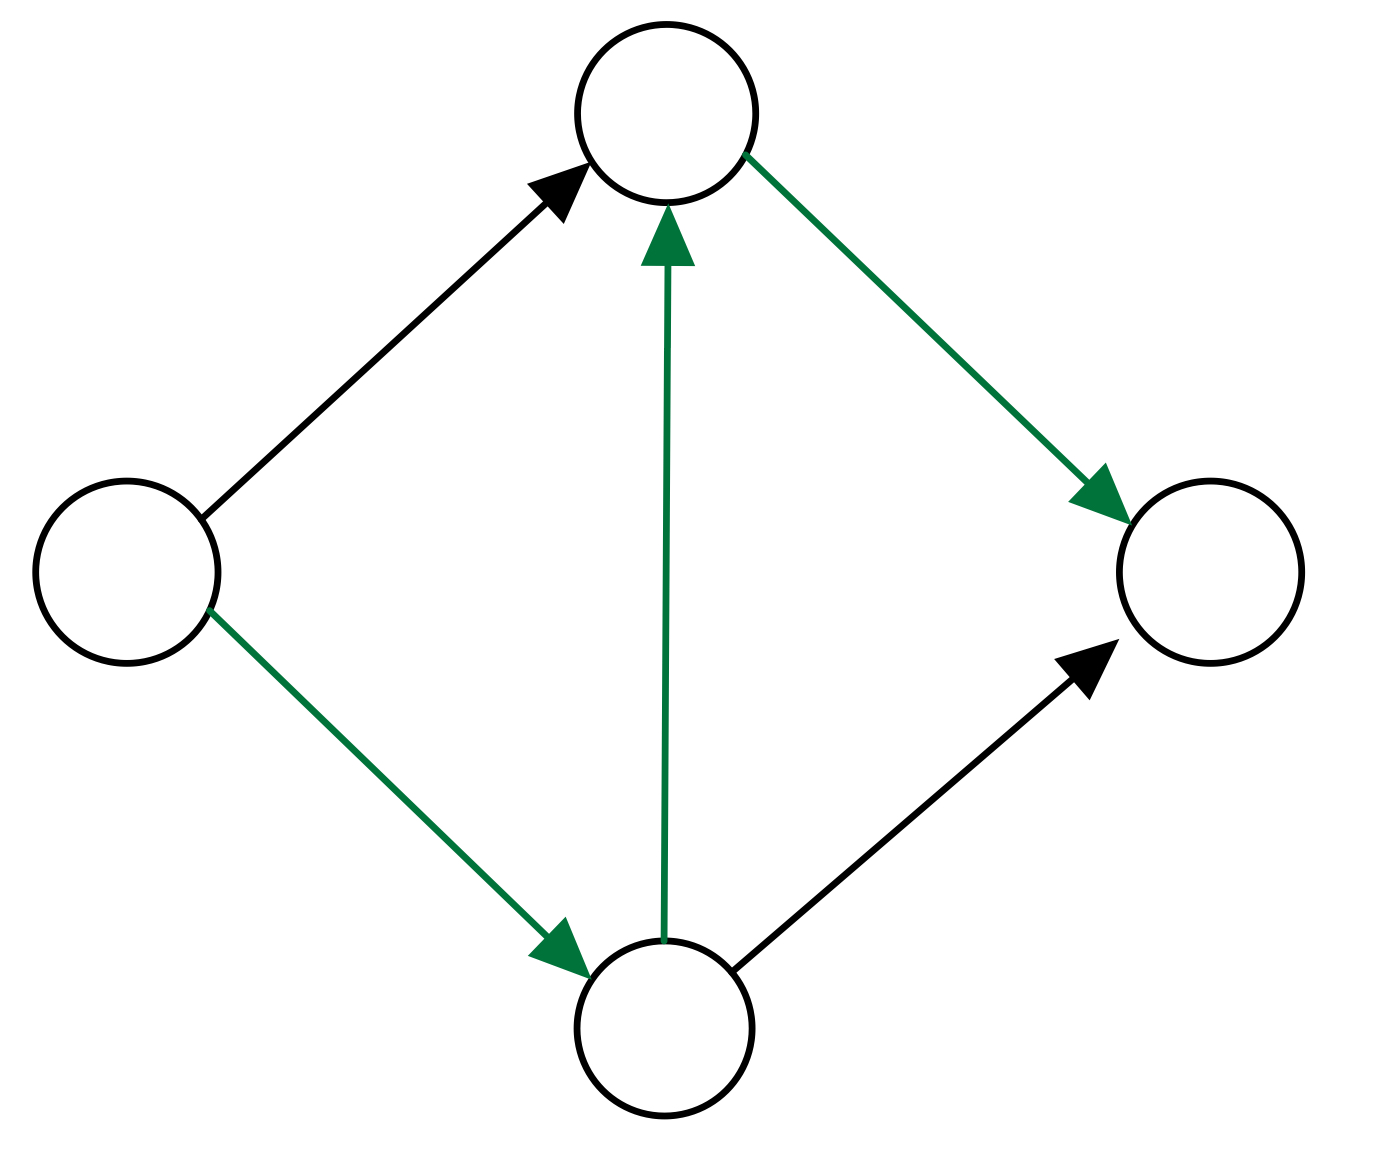
\includegraphics[scale = 0.15]{~/Study/3rdSem/Algorithms/Abstracts/images/lect03/blocking_flow.jpeg}
\end{example}

\begin{note}
	Блокирующий поток совершенно не обязательно наибольший.	
\end{note}

\subsection{Поиск блокирующего потока}

За $O(nm)$ \\

\textit{Забудем что у нас бывают обратные ребра.} \\
Идея проста, будем пускать поток пока получается, а для оптимизации учтем тот факт, что если мы уже однажды пытались пойти вдоль ребра, и узнали что после прохода по нему дойти до $t$ не получится, то нам не стоит идти по этому ребру снова. Это аналог метки used в DFS.

\newpage 

\begin{lstlisting}[language = C++]
	auto first_worthy_edge_num = vector<int>(); 
	/*first_worthy_edge[v] -- relative number of the first edge 
							  which is worth considiring from v. */

	long long dfs(int v, long long flow){
	//If we've followed the path and we can push the flow, we do it.

		if (v == t) return flow;

	//While there is at least one worthy edge.
		while (first_worthy_edge_num[v] < outbound[v].size()){
			auto cur_e = g[v][first_worthy_edge_num[v]];
		
		/*If there is some additional flow we can push and the edge is 
						 presented in initial network (is not reverse). */

		//We will code edge presence checker in Dinic's algorithm.
		if (edges[e].capacity > edges[e].flow && e is not reverse edge){
				auto next_flow = dfs(edges[e].to, 
				                     min(flow, edges[e].cap - edges[e].flow));


				if (next_flow > 0){
					edges[e].flow	 += next_flow;
					edges[e ^ 1].flow -= next_flow;

					return next_flow;
				}
			}
		
			++first_worthy_edge_num[v];
		}

		return 0;
	}
\end{lstlisting}

Тогда сам поиск блокирующего потока будет иметь вид
\begin{lstlisting}[language = C++]
	while ((auto x = dfs(s, inf)) != 0){
		blocking_flow += x;
	}
\end{lstlisting}

Алгоритм работает за $O(nm)$, ведь если главный вызов dfs (из main) суммарно сдвинул все номера интересных вершин на $k$, то dfs работал  $n + k$, так как каждое ребро либо нас устроило, и мы просто увеличили номер, либо оно нас устроило, и мы пошли в новую вершину, а сдвигать указатели долго мы не сможем, суммарно сдвигов будет не больше чем  $m$, а значит время работы $ =  n * $ кол-во запусков $+ m$, а каждый запуск насыщает хоть 1 ребро, при этом из-за отсутствия обратного ребра, ребра не рассыщаются. Значит имеем асимптотику  $O(nm)$

\subsection{Алгоритм Диница для поиска наибольшего потока }

За $O(n^2 m)$ \\

Пусть $G$ -- сеть. \\
$dist(s, v)$ -- кратчайшее расстояние между вершинами. \\

Определим слоистую сеть: \\
Вершина s. \\
Вершины с $dist$ 1 от s. \\
	... \\
Вершины на расстоянии k от s. \\

При этом оставим только ребра, идущие из меньшего уровня в следующий по порядку, то есть кратчайшие пути.

\textbf{Алгоритм} \\
\textit{Вспомним что у нас бывают обратные ребра.}\\
Пока не найден наибольший поток:
\begin{enumerate}
	\item Построим слоистую сеть.
	\item Пустим в ней произвольный блокирующий поток.
\end{enumerate}

\begin{prop}
	Алгоритм Диница находит наибольший поток.	
\end{prop}

\begin{proof} \ \\
	Теорема Форда-Фалкерсона учит нас что поток максимален $\iff$ в остаточной сети нет увеличивающего пути. Если наш алгоритм завершился, то есть не сумел пустить блокирующий поток в слоистой сети, значит в слоистой сети нет пути из $s$ в  $t$, а по построению слоистой сети, это значит что и в исходной сети пути из $s$ в  $t$.
\end{proof}

\begin{prop}
	Алгоритм Диница делает не более $n$	итераций.
\end{prop}

\begin{proof} \ \\
	Покажем что после каждой итерации $dist'(s, t) > dist(s, t)$. \\
	На каждом пути из $s$ в  $t$ есть хоть одно насыщенное ребро, ведь мы пустили блокирующий поток. (По определению блокирующего потока) \\
	После того как мы пустили блокирующий поток, у в слоистой сети исчезли некоторые ребра слева направо, а обратные ребра справа налево наоборот появились, значит расстояние в слоистой сети увеличилось, а значит увеличилось и расстояние в исходной сети.
\end{proof}


\subsection{Теоремы Карзанова.}%
\label{sub:Теоремы Карзанова.}

Зачастую асимптотика алгоритма Диница завышена, так как сеть в задаче имеет специфичный вид. Теоремы Карзанова помогают точнее оценить число итераций.

\begin{Def}
	\textbf{$C_{out}(v)$} $= \sum\limits_{u \in V} cap(v, u)$
	\textbf{$C_{in}(v)$} $= \sum\limits_{u \in V} cap(u, v)$
\end{Def}

\begin{note}
	Понятно что тогда через любую вершину течет не более чем $min(C_{in}(v), C_{out}(v))$
\end{note}

\begin{Def}
	\textbf{Общий потенциал сети $P$} $= \sum\limits_{v \in V, v \neq s, t} min(C_{out}(v), C_{in}(v))$
\end{Def}

\begin{lemma}
	В сети $G$ $l = dist(s, t) \leq \frac{P}{F} + 1$, где $F$ -- максимальный поток, $P$ -- общий потенциал. 
\end{lemma}
\begin{proof} \ \\
	Пусть $V_i = \{v: dist(s, v) = i\}$ \\
	Получилась слоистая сеть, в которой ребра есть только из  $V_i$ в  $V_{i + 1}$ \\
	Таким образом, если разрез и пересекает какое-либо ребро, то оно идет между слоями \\
	A cумма capacity ребер между слоями не меньше чем максимальный поток. \\ 
	$cap(\cup_0^i V_k, \cup_{i + 1}^l V_k) = \sum\limits_{x \in V_i, y \in V_{i + 1}} cap(x, y) \geq F$ \\
	Просуммируем это неравенство по всем $i$: \\
	$\sum\limits_{i = 0}^{l - 1} \sum\limits_{x \in V_i, y \in V_{i + 1}} cap(x, y) \geq (l - 1)F$ \\
	А сверху эту сумму можно оценить общим потенциалом сети, ведь сумма capacity ребер между слоями не может превышать сумму capacity ребер в одном слое, которая, в свою очередь, не превышает сумму потенциалов вершин в $V_i$. \\
	$P \geq (l - 1)F$
\end{proof}

\begin{lemma}
	После проталкивания потока $f$	в сети $G$, общий потенциал остаточной сети  $G_f$ равен общему потенциалу исходной сети.
\end{lemma}
\begin{proof} \ \\
	Когда мы проталкиваем поток $f$ вдоль ребер $(u, v)$ и $(v, w)$ по обратным ребрам проходит $-f$. \\
	Таким образом уменьшение $C_{in}(v)$ за счет потока по $(u, v)$ будет скомпенсировано увеличением  $C_{in}(v)$ за счет увеличения потока по обратному ребру  $(w, v)$.
\end{proof}

\begin{theorem}
	Число итераций алгоритма Диница в сети $G$ с целочисленными capacity --  $O(\sqrt{P})$
\end{theorem}
\begin{proof} \ \\
	Сделаем ровно $\sqrt{P}$ итераций, тогда $l \geq \sqrt{P}$, ведь, как мы уже знаем, каждая итерация увеличивает расстояние между $s$ и $t$ хоть на 1. \\
	Запишем утверждение первой леммы для остаточно сети после $\sqrt P$ итераций: \\
	$l \leq  \frac{P}{F_{ост}} + 1$, а $F_{ост} = F - f$, где $f$ -- то сколько потока удалось протолкнуть за прошедшие итерации. \\
	При это $f \geq \sqrt P$, ведь все capacity целочисленные, и мы не могли проталкивать меньше 1 единицы потока за итерацию. \\
	Таким образом получаем $F \leq 2\sqrt{P}$ 
\end{proof}

	\section{Строки.}%


\subsection{Совпадение подстрок в строке.}%

Построим \textbf{полиномиальную} хеш-функцию, которая каждой строке в соответствие ставит число.
\[h_{p, m}(\overline{c_{0}c_{1}...c_{n}}) = (c_0 \cdot p^{n - 1} + c_1 \cdot p^{n-2} + ... + c_{n - 2} \cdot p + c_{n - 1}) \ \% \ m\]

При помощи схемы Горнера, такая функция считается за линейное время, ведь $h_{p, m}(\overline{c_{0}c_{1}...c_{n}}) = (...(((c_0 \cdot p + c_1))p + c_2)p + c_3)...)p + a_{n-1}$

Так как мы имеем дело с подстроками одной большой строки, мы можем сделать предподсчет хеш-функции для всех префиксов большой строки, а дальше воспользоваться свойством хеша:
\[
	h(S[l, r)) = (h(S[0, r)) - h(S[0, l)) \cdot p^{r - l + 1}) \ \% \ m
.\] 

Таким образом, после линейного предподсчета, мы можем сравнивать строки по их хешу за константное время.


\subsection{Алгоритм Рабина -- Карпа для поиска подстроки в строке.}%

Для поиска подстроки $S$ длины $m$ в тексте $T$ длины $n$, 
\begin{enumerate}
	\item Подсчитаем $h(T[0, m))$ и $h(S[0, m))$, а также $p^m$.
	\item В цикле по всем $i$ от  $0$ до $n - m$
		\begin{enumerate}
			\item Считаем $h(T[i, m + i))$ и сравниваем его с $h(S[0, m))$. 
			\item В случае равенства, опционально, можно провести проверку наивным посимвольным сравнением или выборочным сравнением символов, для исключения малейшей вероятности коллизии.
		\end{enumerate}
\end{enumerate}

Алгоритм работает за линейное время $O(n + m)$, однако он не устойчив перед коллизиями хеш-функции, дополнительная обработка которых увеличивает время работы.


\subsection{Алгоритм Кнута -- Морриса -- Пратта для поиска подстроки в строке.}%

\subsubsection{Префикс-функция}
Введем для строки $S$ префикс-функцию $\pi$ 
\[
	\pi(i) = \max \limits_{k \in [0, i]} \{k: S[0, k) == S[i + 1 - k, i +1)\}
\]
-- длина наибольшего собственного суффикса подстроки S[:i], который равен префиксу такой же длины. $\pi(0) = 0$ по определению.

\begin{example}
	$S = "adam"$. 
	$\pi(0) = 0$. \\
	$\pi(1) = 0$, ведь у строки  $"a"$ есть только пустой собственный суффикс. \\
	$\pi(2) = 0$, ведь у строки $"ab"$ нет собственного суффикса, совпадающего с префиксом той же длины. \\
	$\pi(3) = 1$, ведь у строки  $"ada"$ есть собственный суффикс  $"a"$ длины 1, который совпадает с префиксом  $"a"$. \\
	$\pi(4) = 0$. \\
\end{example}

Нетрудно представить себе наивный алгоритм, подсчитывающий префикс-функцию строки за $O(n^3)$. Оптимизируем его.



 \begin{prop}
	 $\pi(i + 1) \leq \pi(i) + 1$
\end{prop}
\begin{proof}
	Рассмотрим суффикс, оканчивающийся на позиции $i + 1$ и имеющий длину $\pi(i + 1)$. Удалив из него последний элемент, мы получим суффикс, оканчивающийся на позиции $i$ и имеющий длину  $\pi(i + 1) - 1$\\
	Однако, мы определили $\pi(i)$ максимальную длину суфикса  $\Rightarrow$ $\pi(i) \geq \pi(i + 1) - 1$.
	\begin{center}
		\framebox{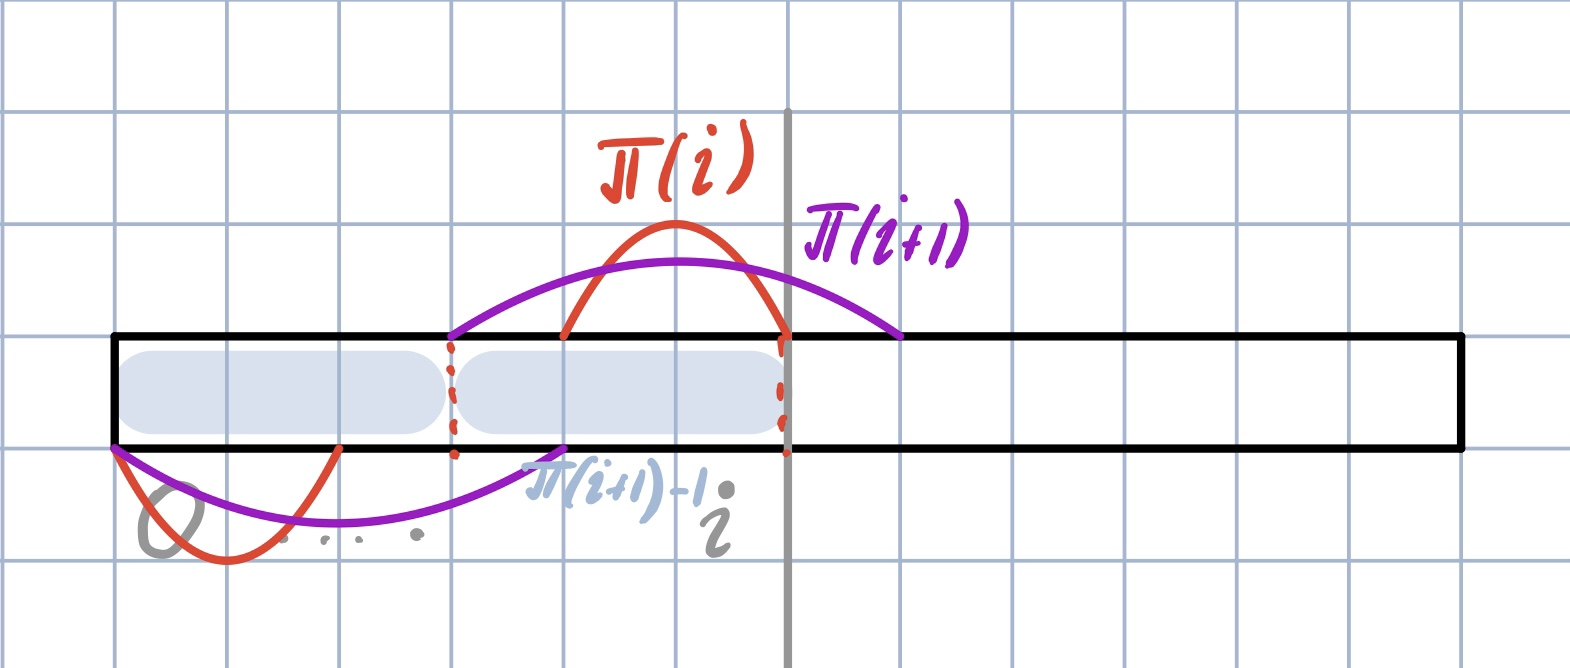
\includegraphics[scale = 0.1]{~/Study/3rdSem/Algorithms/Abstracts/images/lect05/dec_pi_leq.jpeg}}
	\end{center}
\end{proof}

\begin{prop}
	Если $S[\pi(i)] == S[i + 1]$, то  $\pi(i + 1) == \pi(i) + 1$.
\end{prop}
\begin{proof}
	Условие говорит нам, что после префикса длины $\pi(i)$ находится символ, который совпадает с символом, который находится после суффикса, оканчивающегося на позиции $i$. То есть наибольший суффикс, заканчивающийся на позиции $i + 1$ содержит в себе все символы суффикса, заканчивающегося на позиции $i$ и еще один символ. Это и записано в правой части.
	\begin{center}
		\framebox{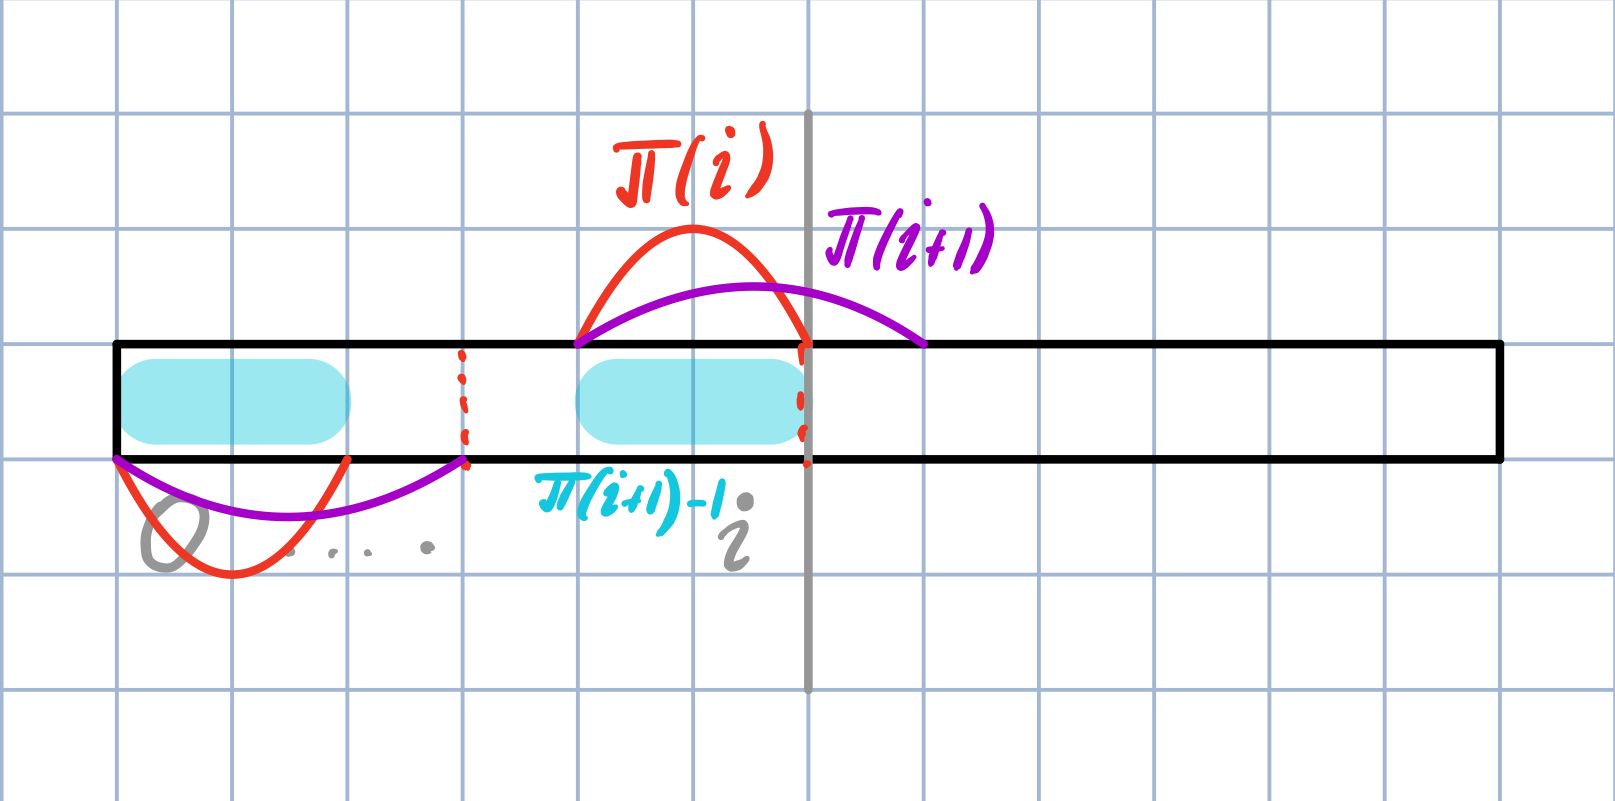
\includegraphics[scale = 0.1]{~/Study/3rdSem/Algorithms/Abstracts/images/lect05/dec_pi_i_plus_1.jpeg}}
	\end{center}
\end{proof}

Пользуясь вторым свойством, мы сможем частично оптимизировать подсчет. Если же окажется что условие равенства символов не выполняется, мы будем искать суффикс меньшей длины следующим образом:
Мы знаем, что $S[1, \pi(\pi(i)))$ -- суффикс подстроки  $S[1, i)$ \\

\textbf{Тогда подсчет можно свести к циклу}
\begin{enumerate}
\setcounter{enumi}{0}
	\item $k = \pi(i)$.
	\begin{enumerate}
		\item Если $S[i + 1] == S[k]$, то $\pi(i + 1) = k + 1$.
		\item Если же $k == 0$, то $\pi(i + 1) = 0$.
	\end{enumerate}
	\item $k = \pi(k)$. Перейти к пункту 1.
\end{enumerate}

Теперь мы будем проходиться по строке, и для каждой позиции вычислять $\pi(i)$ оптимизированно.

\begin{prop}
	Оптимизированный алгоритм подсчета префикс-функции имеет асимптотику $O(n)$.	
\end{prop}
\begin{proof}
	Из вышедоказанного утверждения мы знает что на каждой итерации по индексу строки, $k$ увеличивается не более чем на 1.
\end{proof}

\subsubsection{Z-функция}

Введем для строки $S$ Z-функцию $z$ 
\[
	z(i) = \max \{k: S[i, i + k) == S[0, k)\}
\]
-- длина наибольшей подстроки S, начинающейся с позиции $i$, которая равна префиксу S такой же длины, $z(0) = 0$ по определению.

\begin{example}
	$S = "adam"$. 
	$z(0) = 0.$
	$z(1) = 0.$
	$z(2) = 1.$ 
	$z(3) = 0.$
\end{example}

\begin{Def}
	\textbf{Z-блок} --- подстрока $S$, начинающаяся с позиции  $i$ длины  $z(i)$.
\end{Def}

\textbf{Для построения Z-функции} строки $S$ будем на каждом шаге хранить самый правый  Z-блок -- тот, у которого правая граница является самой правой.
Назовем позиции начала и конца самого правого Z-блока $l$ и  $r$ соответственно. Изначально $l = r = 0$. 

Пусть у нас подсчитана Z-функция и Z-блок для всех позиций $< i$, тогда найдем  $z(i)$.

Рассмотрим 2 случая. 
\begin{enumerate}
	\item \underline{$i \notin [l; r)$}: \\
		Тогда нам придется считать функцию наивно, пробегая двумя указателями по строке с начала и по подстроке, начиная с позиции $i$. Тогда значение $z(i)$ будет определено как первая позиция $j$, такая что  $S[j] != S[i + j]$.
		После этого обновим сохраненное значение самого правого Z-блока.
	\item \underline{$i \in [l, r)$}: \\
		Тут возможны 2 варианта:
		\begin{enumerate}
			\item \underline{$z(i - l) < r - l$}. То есть наибольшая подстрока, начинающаяся с позиции $i - l$, равная префиксу такой же длины, не превышает по длине самый правый Z-блок. \\
				Заметим, что позиция $i - l$ будет лежать в префиксе, равном по длине самый правый Z-блоку. \\
				Тогда $z(i) = z(i - l)$. \\
		\item \underline{$z(i - l) > r - l$}. В этом случае наибольшая подстрока, начинающаяся с позиции $i - l$ выходит за пределы префикса, соответствующего самому правому Z-блоку. \\
				Тогда скажем  что $z(i) = r - i + l$ --- длина той части наибольшей подстроки, начинающейся с позиции  $i - l$, которая лежит внутри префикса, соответствующего самому правому Z-блоку. \textbf{А затем будем наивно улучшать оценку, проходясь по строке начиная с позиции r.}
		\end{enumerate}
\end{enumerate}

\begin{prop}
	Асимптотика вычисления Z-функции --- $O(m)$, где $m$ --- длина строки.
\end{prop}
\begin{proof}
	Каждая позиция в строке просматривается не более двух раз. При попадании в промежуток $[l; r)$ и наивном улучшении, или же в противном случае при непопадании в промежуток и наивном просчете. При этом, всякий раз когда мы считаем Z-функцию наивно, мы обновляем самый правый Z-блок, то есть сдвигаем его правую границу, а это может происходить не более $m$ раз. Значит мы тратим $O(m)$ на базовые операции и $O(m)$ на суммарные наивные проверки.
\end{proof}

\newpage

\subsubsection{Алгоритм}
Для поиска подстроки $S$ длины $m$ в тексте  $T$:
\begin{enumerate}
	\item Построим строки вида $S\#T$, где $\#$ --- произвольный разделитель, не встречающийся в тексте.
	\item По сконструированной строке построим префикс-функцию или Z-функцию.
	\item Тогда если в некоторой позиции  $i$ $\pi(i) == m$, то эта позиции --- конец вхождения подстроки. \\
		Аналогично, если $z(i) == m$, то эта позиция --- начало вхождения подстроки.
\end{enumerate}

\begin{prop}
	Алгоритм работает за $(\lvert S \rvert + \lvert T \rvert)$.
\end{prop}
\begin{proof}
	Ведь Префикс-функция и Z-функция строятся за линейное время, а затем совершается только один проход всей результирующей строки.	
\end{proof}

	\section{Продолжение строк. Алгоритм Ахо -- Корасик для нахождения всех вхождений набора подстрок.}%
Мы хотим научиться искать все вхождения строк из набора в некотором тексте.

\subsection{Построение бора.}%
\begin{Def}
	\textbf{Бор} --- дерево, в котором каждая вершина обозначает строку, а каждое ребро обозначает букву. Строка, соответствующая вершине (то есть заканчивающаяся в этой вершине), получается конкатенацией всех букв, соответствующих ребрам пути из корня в эту самую вершину. По определению, корню бора соответствует пустая строка.
\end{Def}

\begin{Def}
	\textbf{Терминальная вершина} бора для набора слов --- вершина, которой соответствует слово из этого набора.
\end{Def}


Для добавления строки в бор мы: \\
Прочитав очередной символ в цикле по строке, переходим по соответствующему ему ребру или создаем такое ребро если потребуется. \\
После завершения строки помечаем последнюю вершину как терминальную.

Таким образом, бор строится за линейное по сумме всех строк в наборе время.

\subsection{Преобразование бора в автомат.}%
Будем понимать вершины бора и соответствующие им строки как состояния конечного детерминированного автомата. Однако мы сталкиваемся с проблемой, ребер бора не достаточно для отражения всех возможных переходов между состояниями автомата. 
\begin{example}
	Ребра бора не отражают тот факт, что перейдя под воздействием символов $"ad"$ в некоторое состояние  $S_1$ мы все еще можем перейти в состояние  $S_2$.
    \begin{center}
        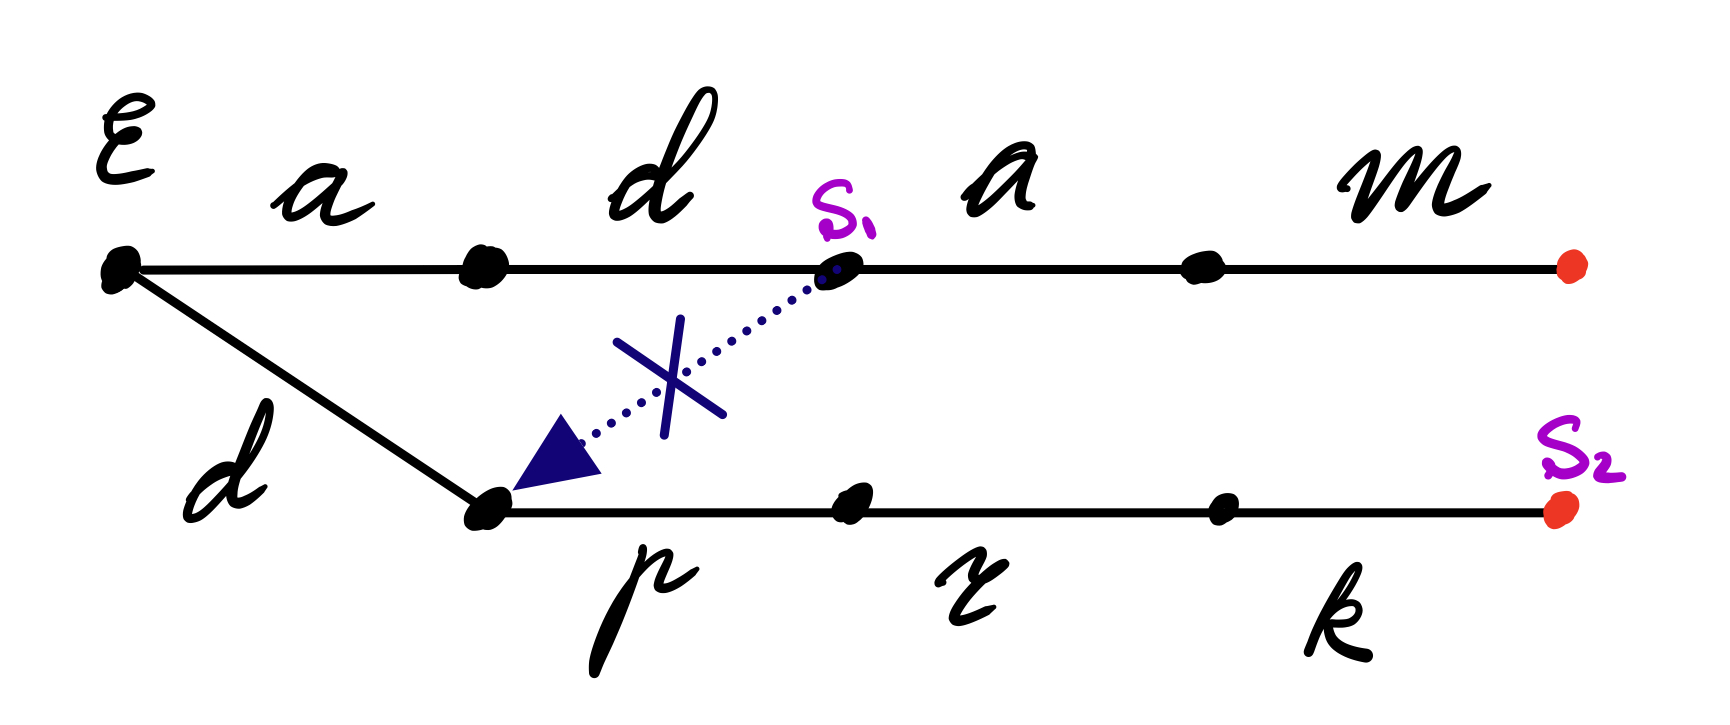
\includegraphics[scale = 0.2]{images/lect06/adam_dprk.jpeg}
    \end{center}
\end{example}

\begin{Def}
	\textbf{Суффиксная ссылка} вершины $v$ --- ссылка (мнимая стрелка в боре) на вершину $u$, такую, что состояние $u$ --- наибольший собственный суффикс состояния $v$, а если такой вершины  $u$ нет, то ссылка на корень. По определению, ссылка из корня ведет в корень.
\end{Def}

\begin{example}
	Для бора строк $"adam"$ и $"dprk"$ единственной суффиксной ссылкой, не ведущей в корень, будет ссылка из состояния $"ad"$, в состояние $"d"$, зачеркнутая на рисунке выше.
\end{example}

\subsubsection{Нахождение суффиксных ссылок.}

\textbf{Чтобы найти суффиксную ссылку} для вершины $v$:  \\
Если $v$ -- корень, то и его суффиксная ссылка тоже корень.
В противном случае: \\
\begin{itemize}
\item Пусть $c$ --- буква, преводящая из родителя в вершину $v$. 
\item Рассмотрим в качестве текущей вершины суффиксную ссылку родителя. 
\item Пока в рассматриваемой вершине нет ребра, соответствующего букве $c$, будем прыгать дальше, рассматривая ее суффиксную ссылку. 
\item Если мы уперлись в корень, то корень и является суффиксной ссылкой вершины $v$. 
\item Если мы нашли вершину $u$, с ребром  $c$, то суффиксной ссылкой будет вершина, в которую ребро  $c$ переводит  вершину $u$.
\end{itemize}

Концептуально, мы берем наибольший собственный суффикс родителя и откусываем от него по одной букве слева, пока не получится подстрока, которая добавлением одного символа становится собственным суффиксом нашей исходной строки.

\begin{lstlisting}[language = C++]
    auto get_suflink(Node_t* node){
        
        if (node == root) return root;

        auto last_c = node->c;
        auto parent = node->parent;

        while(parent != root && parent->go[last_c] == nullptr){
            parent = get_suflink(parent);
        }

        if (parent == root) return root;
        return parent->go[last_c];
    }
\end{lstlisting}

Этот алгоритм терминируется, ведь на каждом шаге мы поднимаемся выше по бору, а значит рано или поздно дойдем до корня.

Мы считаем суффиксные ссылки рекурсивно, но этот процесс можно \textbf{оптимизировать, записав суффиксную ссылку в вершину}, ведь после построения автомата она меняться не будет.
Тогда мы можем ввести универсальную автоматную функцию перехода, которая не делает различия между суффиксными ссылками.

$jump(node, c) = $
\begin{itemize}
    \item[$\textperiodcentered$] $son\_c$, \text{если ребро бора $c$ переводит вершину $node$ в  $son\_c$}
    \item[$\textperiodcentered$] $null$, \text{если $node$ --- корень, у которого нет ребра бора $c$}
    \item[$\textperiodcentered$] $go(suflink(node), c)$, \text{иначе}
\end{itemize}

С учетом концепции универсальности перехода, переход по суффиксной ссылке вершины --- переход из суффиксной ссылки родителя по ребру $c$, где  $c$ --- ребро, которое перевело родителя в вершину.
\begin{lstlisting}[language = C++]
    suflink(node) = jump(suflink(node->parent), node->c); 
\end{lstlisting}

Тогда чтобы посчитать суффиксные ссылки мы пойдем по дереву по слоям, высчитывая suflink и jump одновременно:
\begin{enumerate}
    \item Для корня все известно.
    \item Для первого слоя suflink ведет в корень, а jump вниз или по suflink в корень и по go от него.
    \item Для каждого из следующих уровней мы можем найти и suflink и jump за $O(1)$, ведь для родителя, который находится уровнем выше мы уже все посчитали.
\end{enumerate}
Концептуально это BFS.

\subsection{Поиск вхождений при помощи автомата.}
Для поиска набора строк в тексте:
\begin{enumerate}
    \item Построим автомат по набору строк. 
    \item Каждый раз будем считывать букву текста, и совершать переход по ней в автомате.
\end{enumerate}
При этом, мы поймем, что нашли совпадение строки из набора, если текущая вершина терминальная, \textit{а также если, двигаясь по суффиксным ссылкам, мы можем достигнуть терминальной вершины.} \\
Из-за этого отягчающего обстоятельства, определение вхождения строки в текст для каждого состояния будет занимать линейное время.
Оптимизируем это движение по суффиксным ссылкам.

\subsection{Нахождение сжатых терминальных ссылок.}
\begin{Def}
    \textbf{Сжатая терминальная ссылка} вершины $v$ --- ближайшая достижимая по суффиксным ссылкам из $v$ вершина$w$, являющаяся терминальной и не совпадающая с $v$.
\end{Def}

\begin{example} 

Сжатые терминальные ссылки отмечены синим.
\begin{center}
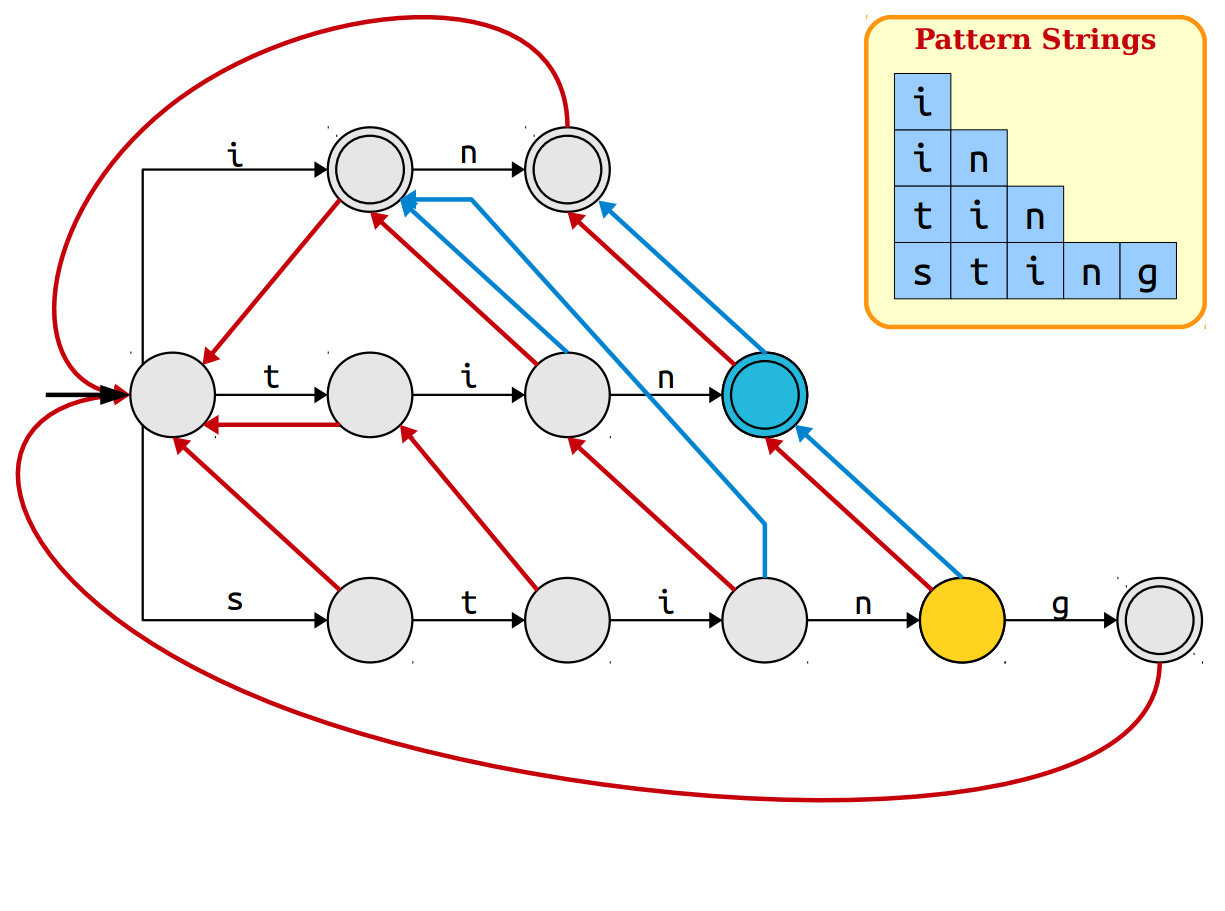
\includegraphics[scale = 0.3]{"images/lect06/Aho-Corasick-complete-links.png"}
\end{center}
\end{example}

Концептуально, сжатые терминальные ссылки собирают в односвязный список все терминальные вершины, а значит и все подстроки, вхождение которых имело место при достижении текущего состояния.
Таким образом, учитывая что сжатая терминальная ссылка ведет только наверх, мы сможем построить эти ссылки по слоям при помощи BFS.
\newpage
\begin{lstlisting}[language = C++]
    if (suflink(node)->is_terminal){
        complete_link(node) = suflink(node);
    }

    else {
        complete_link(node) = complete_link(suflink(node));
    }
\end{lstlisting}

\subsection{Алгоритм с использованием сжатых терминальных ссылок.}
\begin{enumerate}
    \item Построим автомат по набору строк.
    \item Построим сжатые терминальные ссылки в автомате.
    \item Для каждого считанного символа $c$:
        \begin{enumerate}
            \item $cur\_node = go(root, c)$
            \item Если $cur\_node == null$, вхождение соответствует, идем дальше.
            \item В противном случае, засвидетельствуем вхождение подстроки, соответствующей текущей вершине, если она терминальная, а также всех ее сжатых терминальных ссылок.
        \end{enumerate}
\end{enumerate}

\subsection{Сложность алгоритма.}
Пусть $\Sigma$ --- суммарная длина подстрок в наборе,  $T$ --- длина текста, по которому осуществляется поиск, $Ans$ --- число найденных вхождений.

\begin{enumerate}
    \item Построение бора требует $O(\Sigma)$
    \item Построение суффиксных ссылок, по сути, BFS по дереву, требует  $O(\Sigma)$
    \item Построение сжатых терминальных ссылок, также BFS по дереву, требует $O(\Sigma)$
    \item Цикл по каждому из символом --- $O(T)$
    \item Проходы по сжатым терминальным ссылкам суммарно займут  $O(Ans)$
\end{enumerate}

Итого, имеем $O(\Sigma + T + Ans)$

    
%    \newpage
\section{Additional information}


\end{document}
